\section{Integrator und Differentiator}
Dieser Versuch dient der praktischen Untersuchung einer Integratorschaltung mittels
Operationsverst\"arker.
\subsection{Experimentelle Durchf\"urung}
In diesem Versuch wird ein Integrator wie in Abbildung 8 zu sehen ist, aufgebaut. Dabei werden folgende Werte verwendet:
\begin{eqnarray*}
R_1 &=& 1~k\Omega\\
C &=& 150~nF\\
f &=& 1~kHz
\end{eqnarray*}
Als Eingangssignal sollen verschiedene Kurvenform verwendet werden. Die Ausgangssignale f\"ur jeder Kurvenform sind im Ergebnisteil dargestellt. 
\begin{figure}[!ht]
\begin{center}
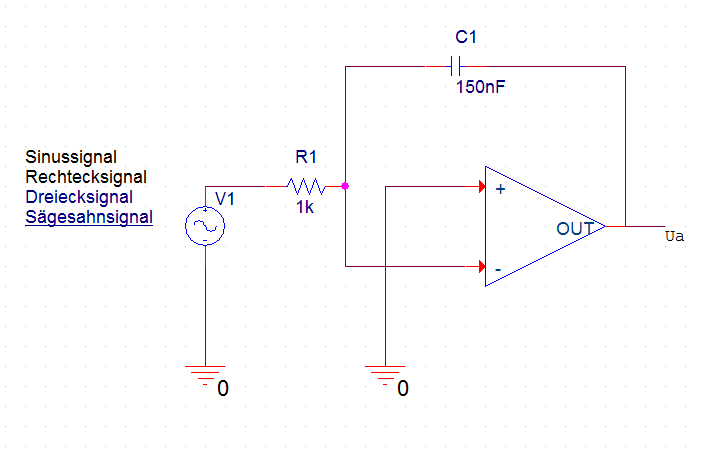
\includegraphics[scale=0.6]{bild/integrierer}
\caption{Sinussignal am Integrator}
\end{center}
\end{figure}
\newpage
\subsection{Ergebnisse und Diskussion}
Das integrierende Verhalten der Integrator-Schaltung ist in den Abbildungen 9 bis 12 gut zu erkennen.\\
Die Eingangsspannung ist jeweils blau und die Ausgangsspannung ist jeweils gelb.
\begin{figure}[!h]
\begin{minipage}{0.4\textwidth}
\begin{center}
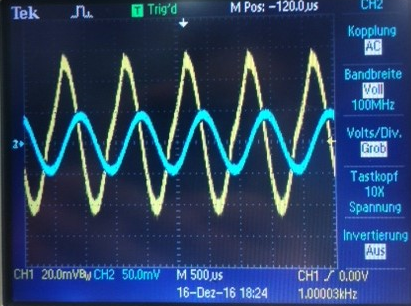
\includegraphics[scale=0.6]{bild/image5}
\caption{Sinussignal am Integrator}
\end{center}
\end{minipage}
\hfill
\begin{minipage}{0.4\textwidth}
\begin{center}
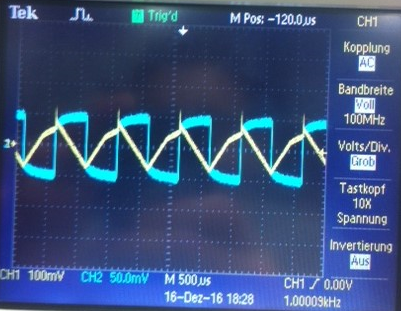
\includegraphics[scale=0.6]{bild/image6}
\caption{Rechtecksignal am Integrator}
\end{center}
\end{minipage}
\end{figure}
\begin{figure}[!ht]
\begin{minipage}{0.4\textwidth}
\begin{center}
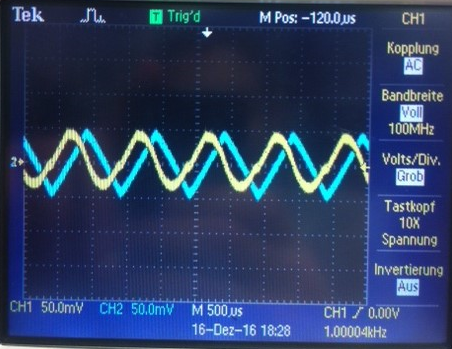
\includegraphics[scale=0.6]{bild/image7}
\caption{Dreiecksignal am Integrator}
\end{center}
\end{minipage}
\hfill
\begin{minipage}{0.4\textwidth}
\begin{center}
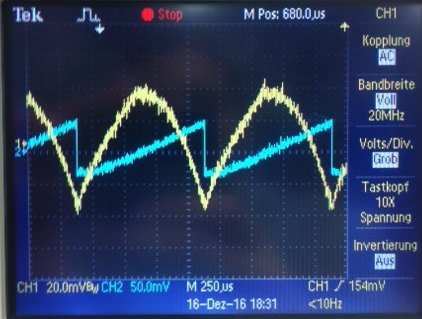
\includegraphics[scale=0.6]{bild/image8}
\caption{S\"agesahnsignal am Integrator}
\end{center}
\end{minipage}
\end{figure}

\newpage
\begin{figure}[!ht]
\begin{center}
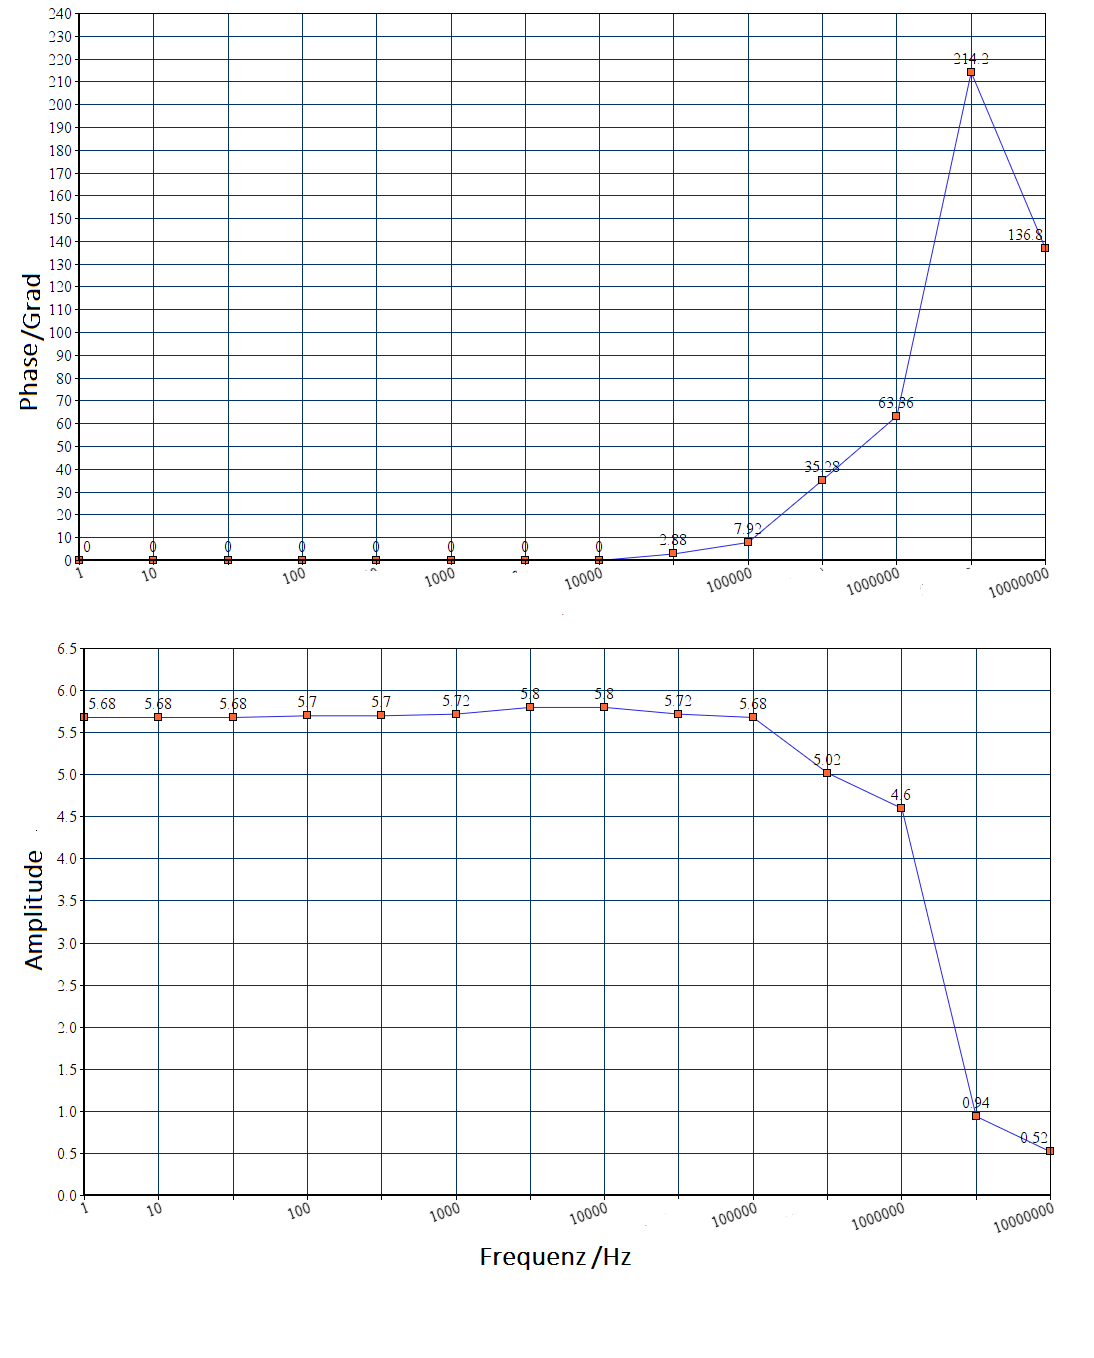
\includegraphics[scale=0.5]{bild/Pahsengang50}
\caption{Phasen- und Amplitudengang mit A=50}
\end{center}
\end{figure}
